\section{Design}
The concept for the GeoLog originally came from Dr. Andrew Wickert (seen in figure 
\ref{fig:andrewWickert}), which came to Reykjavík University's Mechatronics class for 
help developing his design of a low cost, low power datalogger\cite{ALog-BottleLogger}. 
He had two problems needed to be solved. First was to minimize the power consumption of the device he had already developed and the latter was to have means of getting the data
back without having to travel trough difficult terrain. Decision was made to help Andrew 
improve the latter with emphasis on making the system as modular as possible. 

\begin{figure}
\centering
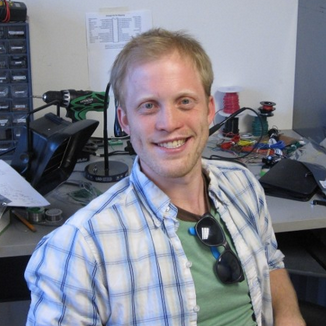
\includegraphics[width=0.4\linewidth]{graphics/andrewWickert}
\caption{Andrew Wickert\label{fig:andrewWickert}\cite{andrewWickert}}
\end{figure}

The GeoLog datalogger was designed in nine phases. Phases seven to eight were iterated
until the product was ready for deployment.

\begin{itemize}
	\item{Phase 1:} Initial brainstorming and high level design phase.
	\item{Phase 2:} Hardware selection phase, where hardware was selected and ordered.
	\item{Phase 3:} Software design phase, where the classes and interfaces were designed.
	\item{Phase 4:} Hardware hacking phase, trial and error in software writing for the
					Wixels\cite{wixel} and the GSM/GPRS module\cite{SM5100B}.
	\item{Phase 5:} Building phase, where hardware were assembled.
	\item{Phase 6:} Software integration phase, all the software integrated to one.
	\item{Phase 7:} Field testing phase, testing of the system in real life environment.
	\item{Phase 8:} Fixing phase, fixing bugs found in the field testing phase.
	\item{Phase 9:} Deployment phase, system is functional and can be deployed. 
\end{itemize}

\textit{\textcolor{red}{Assumptions stated (There are always some)}}


\subsection{Hardware}
\begin{figure}
\centering
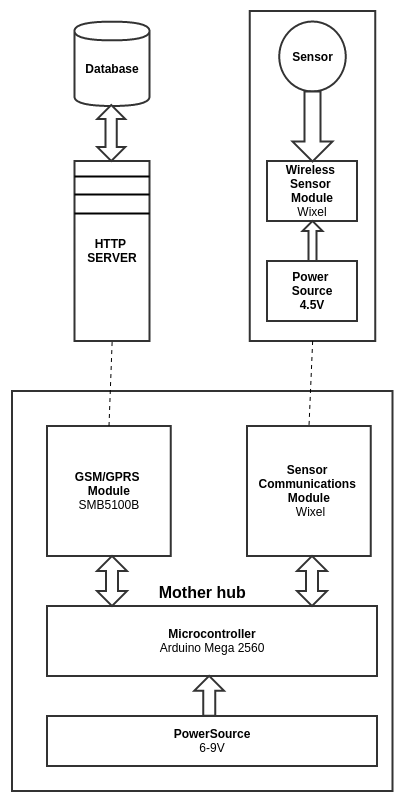
\includegraphics[width=0.5\linewidth]{graphics/HardwareMDD}
\caption{Hardware Module Design Diagram\label{fig:HardwareMDD}}
\end{figure}

The hardware is divided to sensor modules and the mother hub. The sensor modules 
designed for this system were three wireless temperature sensors using Wixel\cite{wixel}
for means of communications. The mother hub consists of a Arduino Mega\cite{arduinoMega}
that communicates with the sensor modules with a Wixel, collects the data 
and sends it to a HTTP server via the GSM/GPRS module\cite{SM5100B}. 
Figure \ref{fig:HardwareMDD} shows how the hardware is set up. 

\subsubsection{Sensor module}
The sensor module is based on Wixel\cite{wixel} that reads sensor value on one of it's
analog inputs when the mother hub calls for reading. To save energy the sensor module does
not send any data until it's id is called by the mother hub. The sensor module then 
gathers several readings from the sensor over a short period of time and sends back the 
average reading of the data collected then falls back to suspend mode until the mother 
hub calls for data again. Electrical schematic diagram of the sensor module can
be seen in figure \ref{fig:sensormodule_schematic}.

\subsubsection{Mother hub}
The mother hub is based on Arduino Mega 2560\cite{arduinoMega} which can be switched out 
for Andrew's Bottle Logger\cite{ALog-BottleLogger}, a Wixel\cite{wixel} used for 
communicating with the wireless sensor modules and a SM5100B GSM/GPRS 
module\cite{SM5100B}. The mother hub gathers data from the Wireless sensor modules via 
the onboard Wixel by calling them by id and wait till corresponding sensor module answers
with newly gathered sensor data. The data gathered is then saved to its onboard EEPROM
and at a preset time the data is sent to HTTP server via GPRS where it can be processed 
by the researcher. Electrical schematic diagram of the mother hub can be seen in figure 
\ref{fig:motherhub_schematic}.

\subsection{Software}
\begin{figure}
\centering
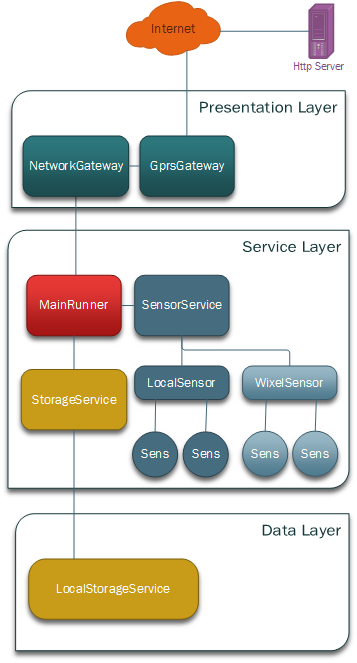
\includegraphics[width=0.6\linewidth]{graphics/Layering}
\caption{Layered Design Diagram of the system\label{fig:Layering}}
\end{figure}

When designing the software, modularity was the main interest. The design aims for making
it as easy as possible to implement new ways of communications, sensors and storage. This 
is done by building the software up of three interfaces the user needs to implement if for
example another means of communications is needed. The system comes with two ways of
communications to the outside world, a SMS gateway and a GPRS HTTP gateway. It comes also with one way of storing data, to the EEPROM and one way of communicating to wireless sensors. Figure \ref{fig:Layering} shows the layered design of the software. 

To take a closer look in to the software and how the interfaces work see the class diagram
shown in figure \ref{fig:ClassDiagram}. Next sections will describe more thoroughly how each 
module works under the hood. All code is written in C++ except the HTTP server which is 
written in Python/Flask-Restful.

\subsubsection{Sensor Service interface}
The sensor service is a interface that developer needs to implement for making a new
sensor module. The sensor service interface has three virtual methods that the developer
needs to implement by inheriting from the SensorService class. The methods in the 
SensorService class that have to be implemented are followed:

\begin{itemize}
	\item \textbf{int getSensorData(int sensorId)}
		\begin{itemize}
			\item Takes in the id of the sensor and returns the raw value.
		\end{itemize}
	\item \textbf{int sendDataToSensor(String data)}
		\begin{itemize}
			\item Takes in data to send to sensor and returns 0 for OK and -1 for error.
				  This could be used to remote calibrate sensor.
		\end{itemize}
	\item \textbf{int setDateTime(long DateTime)}
		\begin{itemize}
			\item Takes in datetime for setting the time on the sensor if needed.
		\end{itemize}
\end{itemize}


\subsubsection{Storage Service interface}

\begin{itemize}
	\item \textbf{int save(String data)}
		\begin{itemize}
			\item Takes in data in String format and saves it to storage medium. 
			      Returns number of bytes saved, returns -1 if not enough space.
		\end{itemize}
	\item \textbf{String load()}
		\begin{itemize}
			\item Loads all data in memory and returns it in string format.
		\end{itemize}
	\item \textbf{int erase()}
		\begin{itemize}
			\item Erases all data from storage medium. Returns number of bytes
			      free after erase.
		\end{itemize}
	\item \textbf{bool isFreeSpcace(int dataSize)}
		\begin{itemize}
			\item Takes in size of data to be saved in bytes. Returns true if enough 
			      space is available, false if not.
		\end{itemize}
\end{itemize}


\subsubsection{Network Gateway interface}

\subsubsection{Main Runner}

\subsubsection{HTTP Server}

\textit{\textcolor{red}{Description of the design; break into pieces and show how 
						they assemble.}}

\textit{\textcolor{red}{Pseudo code of important modules}}

\textit{\textcolor{red}{MDD of structure}}

\textit{\textcolor{red}{System diagram}}

\subsection{Safety}
